\documentclass[%margin%,line,pifont,palatino,courier
]{article}
\usepackage{fullpage}
\usepackage{lastpage}
\usepackage[top=1in,bottom=1in,margin=1in]{geometry}
\usepackage{supertabular}
\usepackage{graphicx,tikz}	
%\usepackage{tkz-euclide}
%\usetkzobj{all}
%\usetikzlibrary{calc}
\usepackage{array,multicol}
\usepackage{amsmath,amssymb}
\usepackage{enumitem}

\usepackage{fancyhdr}
\pagestyle{fancy}

\addtolength{\topmargin}{-0.25in}

\newcommand{\vect}[1]{\mathbf{#1}}
\DeclareMathOperator{\proj}{proj}

\fancypagestyle{plain}{
	\addtolength{\headheight}{0.485in}
	\rhead{\bf MATH 235 (Calculus I) \\
		%\vspace{0.5pc}
		due Tues 19 Sep 2017 \\}
	\rfoot{\footnotesize THQuiz 2, p. \thepage\ (of \pageref{LastPage})
	}
\renewcommand{\headrulewidth}{0pt}
}
\fancyhf{}
\renewcommand{\headrulewidth}{0pt}
\rfoot{\footnotesize THQuiz 2, p. \thepage\ (of \pageref{LastPage})$\;$}

\title{\vspace{-3.5pc} 
	\flushleft \bf \Large Take-Home Quiz 2: Exponentials, Inverses, and Limits %\\ 
	 (\S1.4-1.5, 2.2-2.3)}
\date{}

% % % % %
\begin{document}
\maketitle

\vspace{-3pc}
\noindent{\bf Directions:} This quiz is due on September 19, 2017 at the beginning of lecture.  You may use whatever resources you like -- e.g., other textbooks, websites, collaboration with classmates -- to complete it \textbf{but YOU MUST DOCUMENT YOUR SOURCES}.  Acceptable documentation is enough information for me to find the source myself.  Rote copying another's work is unacceptable, regardless of whether you document it.  

\noindent\hrulefill

\begin{enumerate}
% % %
\item {\bf \S1.4 \#32} An isotope of sodium, $^{\text{24}}$Na, has a half-life of 15 hours.  A sample of this isotope has mass 2g.
	\begin{enumerate}
	\item How much of the sample remains after 60 hours?
	\item Find an exponential function modelling the decay of $^{\text{24}}$Na.
	%\item Find the amount remaining after $t$ hours.
	\item Estimate the amount (round to three decimal places) of the 2g sample remaining after 4 days.
	\item Use a graph (e.g., \verb+desmos.com/calculator+) to estimate the number of days (round to one decimal place) it takes for the 2g mass to be reduced to 0.01g.
	\end{enumerate}

% % %
%\item %\begin{enumerate}
	%\item {\bf \S1.5 \#58}
	%	\begin{enumerate}	
	%	\item What are the values of $e^{\ln{300}}$ and $\ln{e^{300}}$?
	%	\item Use your calculator to evaluate $e^{\ln{300}}$ and $\ln{e^{300}}$.  What do you notice?  Can you explain why the calculator has trouble?
	%	\end{enumerate}
	%\item 
%	{\bf \S1.5 \#76}
%		\begin{enumerate}
%		\item Graph the function $f(x)=\sin(\arcsin x)$ and explain the appearance of the graph.
%		\item Graph the function $g(x)=\arcsin(\sin x)$.  How do you explain the appearance of the graph?
%		\end{enumerate}
	%\end{enumerate}

% % %
\item Simplify each expression and explain why (e.g., with a triangle, the unit circle, trig identities).
	\begin{enumerate}
	%\item $\arctan{\sqrt 3}$
	\item {\bf \S1.5 \#64} $\arctan(-1)$
	%\item $\arcsin(-1/\sqrt 2)$
	\item {\bf \S1.5 \#66} $\arccos(\sqrt 3/2)$
	%\item $\arcsin(\sin(5\pi/4))$
	\item {\bf \S1.5 \#70} $\cos(2\arcsin(5/13))$
	%\item $\tan(\arcsin x)$
	\item {\bf \S1.5 \#72} $\sin(2\arccos x)$
	\end{enumerate}

% % %
\item In the theory of relativity, the mass of a particle with speed $v$ is 
\[
m=f(v)=\frac{m_0}{\sqrt{1-\frac{v^2}{c^2}}}
\] 
where $m_0$ is the rest mass of the particle and $c$ is the speed of light in a vacuum.  
	\begin{enumerate}
	\item {\bf \S1.5 \#20} Find the inverse function of $f$ and explain its meaning.
	\item {\bf \S2.2 \#54} What happens as $v\to c^-$?
	\item {\bf \S2.3 \#56} The Lorentz contraction formula 
	\[
	L=L_0\sqrt{1-\frac{v^2}{c^2}}
	\]
	expresses the length $L$ of an object as a function of its velocity $v$ with respect to an observer, where $L_0$ is the length of the object at rest.  Find $\lim_{v\to c^-}L$ and interpret the result.  Why is a left-hand limit necessary?
	\end{enumerate}

% % %
%\item {\bf 2.2 48}
%	\begin{enumerate}
%	\item Graph the function $f(x)=e^x+\ln|x-4|$ for $0\leq x\leq 5$.  Do you think the graph is an accurate representation of $f$?
%	\item How would you get a graph that represents $f$ better?
%	\end{enumerate}


% % %
%\item Solve for $x$.
%	\begin{enumerate}
%	\item {\bf \S1.5 \#52} $\ln(x^2-1)=3$
	%\item $e^{2x}-3e^x+2=0$
%	\item {\bf \S1.5 \#54} $\ln(\ln x)=1$
	%\item $e^{ax}=Ce^{bx}$, where $a\neq b$
%	\item {\bf \S1.5 \#56} $1<e^{ex-1}<2$
	%\item $1-2\ln x<3$
%	\end{enumerate}
	
% % %
\item {\bf \S2.3 \#66} The figure shows a fixed circle $C_1$ with equation $(x-1)^2+y^2=1$ and a shrinking circle $C_2$ with radius $r$ and center the origin.  $P$ is the point $(0,r)$, $Q$ is the upper point of intersection of the two circles, and $R$ is the point of intersection of the line $PQ$ and the $x$-axis.  
%\vspace{-1pc}
\begin{center}
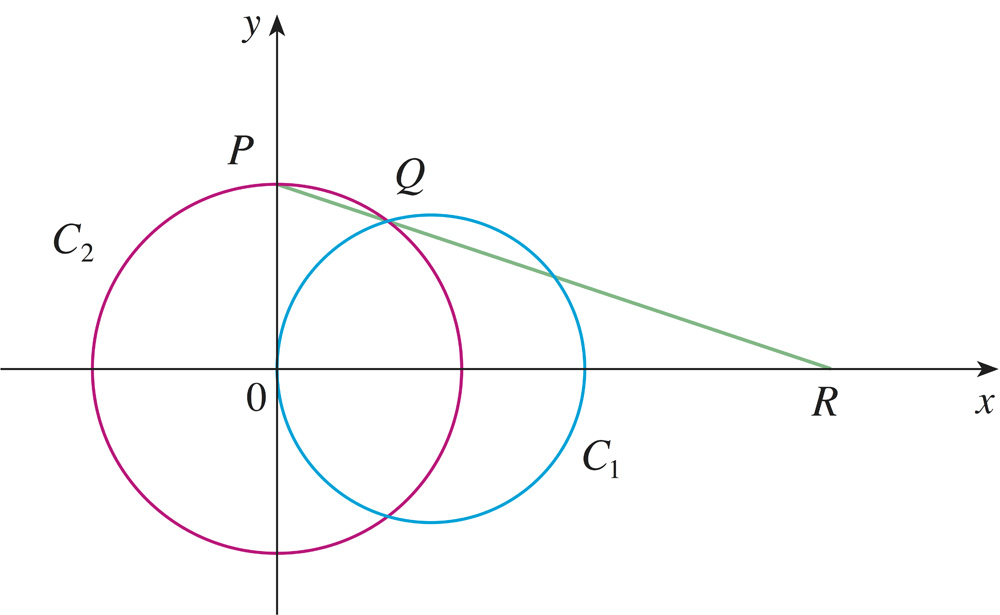
\includegraphics[scale=5]{2-3_66Stewart8Ed}
\end{center}
	\begin{enumerate}
	\item What is the $x$-coordinate of $R$, in terms of $r$?  \emph{(Hint: Find the equation of the line determined by the points $P$ and $Q$.)}
	\item What happens to $R$ as $C_2$ shrinks, that is, as $r\to 0^+$?  \emph{(Hint: Use your answer to part (a).  $R$ does not go to infinity.)}
	\end{enumerate}

% % %
\item {\bf \S2.3 \#60} If $\displaystyle\lim_{x\to 0}\frac{f(x)}{x^2}=5$, find the following limits.  \emph{(Hint: Rewrite $f(x)=\frac{f(x)}{x^2}\cdot x^2$ and $\frac{f(x)}{x}=\frac{f(x)}{x^2}\cdot x$.)}
	\begin{enumerate}
	\item $\displaystyle\lim_{x\to 0}f(x)$
	\item $\displaystyle\lim_{x\to 0}\frac{f(x)}{x}$
	\end{enumerate}

% % %
%\item {\bf 2.3 38} If $2x\leq g(x)\leq x^4-x^2+2$ for all $x$, evaluate $\displaystyle\lim_{x\to 1}g(x)$.

% % %
\item {\bf \S2.3 \#52} Let 
\[
g(x)=\begin{cases}
	x & \text{if }x<1 \\
	3 & \text{if }x=1 \\
	2-x^2 & \text{if }1<x\leq 2 \\
	x-3 & \text{if }x>2
	\end{cases}
\]
	\begin{enumerate}
	\item Evaluate each of the following, if it exists.
		\begin{enumerate}
		\item $\lim_{x\to 1^-}g(x)$
		\item $\lim_{x\to 1}g(x)$
		\item $g(1)$
		\item $\lim_{x\to 2^-}g(x)$
		\item $\lim_{x\to 2^+}g(x)$
		\item $\lim_{x\to 2}g(x)$
		\end{enumerate}
	\item Sketch the graph of $g$.
	\end{enumerate}

% % % % %
\end{enumerate}
\end{document}